\documentclass[bigger]{beamer}

\usepackage{booktabs}
\useinnertheme{rounded}
\usecolortheme{crane}
\setbeamerfont{block title}{size={}}

\title{Experimental Analysis of Mastery Learning Criteria}

\author{\textbf{Radek Pel\'anek} and Ji\v{r}\'i \v{R}ih\'ak\\[10mm]
%Masaryk University Brno\\
%Czech Republic

\includegraphics[width=.3\linewidth]{al-logo}
}

\date{UMAP 2017}
 
\begin{document}

\frame{\titlepage}

\begin{frame}
  \frametitle{Mastery Learning}

  \begin{itemize}
  \item common personalization approach in educational systems
  \item ``practice until mastery, then move to a subsequent topic''
  \end{itemize}
\end{frame}

\definecolor{mygreen}{rgb}{0.0, 0.5, 0.0}
\begin{frame}
  \frametitle{Example}

  \begin{center}
    \begin{tabular}{llll}
      \toprule
      item & answer & time & correct? \\
      \midrule
      $\frac{2}{3} + \frac{4}{5}$ & $\frac{13}{15}$ & 12s & {\color{mygreen}correct}\\[3mm]
      $\frac{3}{4} + \frac{1}{6}$ & $\frac{10}{12}$ & 7s & {\color{red}incorrect}\\[3mm]
      $\frac{2}{7} + \frac{3}{14}$ & $\frac{1}{2}$ & 9s & {\color{mygreen}correct}\\[3mm]
      $\frac{1}{4} + \frac{2}{3}$ & $\frac{11}{12}$ & 7s & {\color{mygreen}correct}\\[3mm]
      $\frac{2}{5} + \frac{3}{7}$ & $\frac{29}{35}$ & 13s & {\color{mygreen}correct}\\[3mm]
      \bottomrule
    \end{tabular}

\medskip

Should the learner continue or move to another topic?
  \end{center}
\end{frame}


% \begin{frame}
%   \frametitle{Mastery Learning}

%   \begin{itemize}
%   \item utilized in many systems...
%   \item our use case Umime cesky
%   \end{itemize}

%   we consider basic setting: single knowledge component, series of binary
%   answers, decide when to stop (and move to another component)
% \end{frame}

\begin{frame}
  \frametitle{Mastery Criteria}

  important, interesting, understudied research direction
  
  \medskip
  
  \begin{itemize}
  \item hard to decide what to use
  \item easy to change in real systems
  \item significant impact on users
  \end{itemize}
\end{frame}


\begin{frame}
  \frametitle{Mastery Criteria}

  \begin{itemize}
  \item \alert{$N$ consecutive correct (NCC)}
  \item moving average
    \begin{itemize}
    \item moving window
    \item \alert{exponential moving average  (EMA)}
    \end{itemize}
  \item based on learner model -- threshold rule 
    \begin{itemize}
    \item \alert{Bayesian knowledge tracing (BKT)}
    \item logistic models
    \end{itemize}
  \end{itemize}

\end{frame}

\begin{frame}
  \frametitle{Evaluation, Thresholds}

  evaluation difficult, no clear ``correct decisions''

  \bigskip

  \begin{center}
    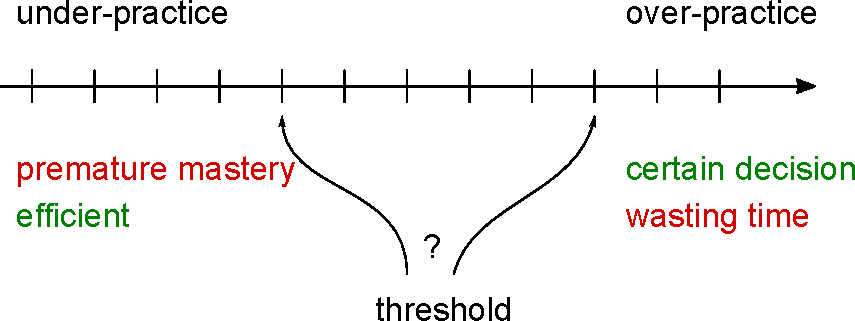
\includegraphics[width=\linewidth]{tradeoff}
  \end{center}

  % \begin{itemize}
  % \item evaluation difficult, no clear ``correct decisions''
  % \item inherent tradeoff: certainty of mastery decision vs. learner's time
  % \item all mastery criteria use some \alert{threshold}
  % \end{itemize}
\end{frame}

\begin{frame}
  \frametitle{Questions}

  \begin{itemize}
  \item Which criterion to use?
  \item Does the use of learner modeling bring advantage?
  \item How to evaluate mastery criteria?
  \item How to choose thresholds?
  \end{itemize}
\end{frame}

\begin{frame}
  \frametitle{Evaluation: Data}

  \begin{itemize}
  \item simulated data
    \begin{itemize}
    \item simplified
    \item ground truth available
    \end{itemize}
  \item real data
    \begin{itemize}
    \item realistic
    \item difficult evaluation
    \end{itemize}
  \end{itemize}
\end{frame}

\begin{frame}
  \frametitle{Results}

  \begin{itemize}
  \item learner models are not fundamental
  \item the choice of thresholds and input data is more important
  \item exponential moving average is a convenient approach
  \end{itemize}
\end{frame}

\begin{frame}
  \frametitle{Importance of Learner Models: BKT vs NCC}

  {\small
  Bayesian knowledge tracing (BKT) vs N consecutive correct (NCC)}

  \smallskip

  \begin{center}
    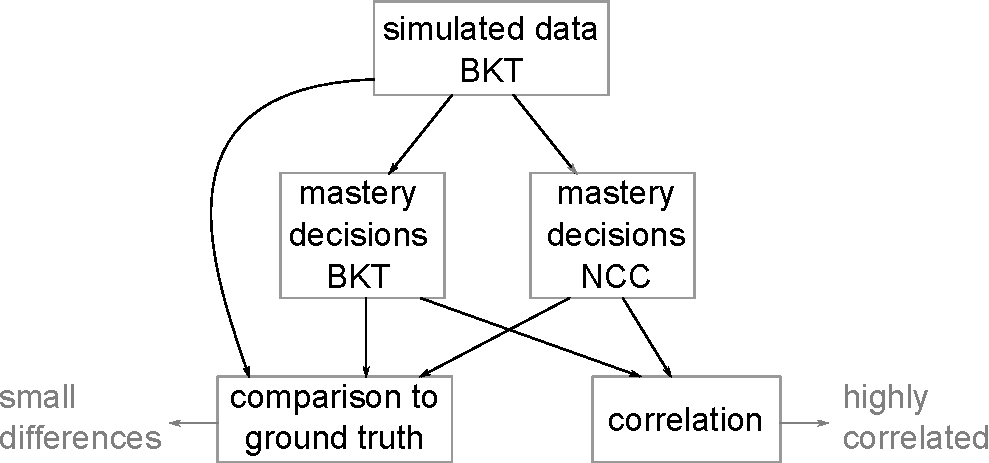
\includegraphics[width=.7\linewidth]{bkt-ncc-experiment}
  \end{center}

  % \begin{itemize}
  % \item simulated data generated by BKT model (optimistic setting for BKT)
  % \item mastery decisions by BKT and NCC:
  %   \begin{itemize}
  %   \item highly correlated (typically $r>0.9$)
  %   \item comparison to ground truth: BKT only slightly better
  %   \end{itemize}
  % \end{itemize}

  \begin{block}{}
    Even under optimistic setting, the learner model does not provide
    fundamental advantage over a very simple mastery criterion.
  \end{block}
\end{frame}

% \begin{frame}
%   \frametitle{Learner Models are not Fundamental}

%   \textbf{BKT vs NCC comparison under data simulated by BKT}

%   \smallskip

%   \begin{center}
%     \begin{tabular}{llllll}
%       \toprule
%       & \multicolumn{2}{c}{Threshold} & \multicolumn{2}{c}{wMAD} & \\
%       &	NCC & BKT &  NCC & BKT & Cor. \\
%       \midrule
%       B1 & 2 & 0.92 & 2.56 & 2.42 & 0.88 \\
%       B2 & 4 & 0.97 & 6.2 & 5.76 & 0.97\\
%       B3 & 2 & 0.95 & 2.81 & 2.48 & 0.92\\
%       B4 & 1 & 0.9 & 2.72 & 2.13 & 0.74\\
%       B5 & 4 & 0.97 & 3.77 & 3.62 & 0.99\\
%       B6 & 8 & 0.97 & 11.48 & 10.33 & 0.94\\
%       \bottomrule
%     \end{tabular}
%   \end{center}
% \end{frame}

\begin{frame}
  \frametitle{Importance of Learner Models: Input Data}

  \begin{center}
  real data (adaptive practice of mathematics)

  \bigskip

    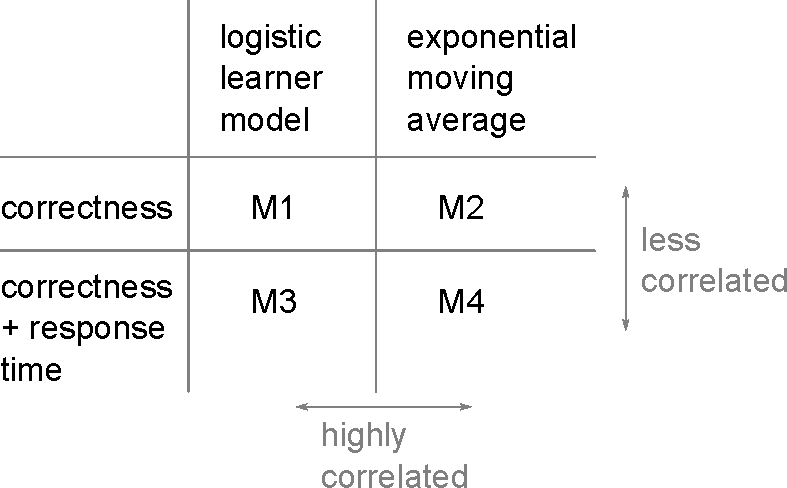
\includegraphics[width=.7\linewidth]{response-time-experiment}
  \end{center}


  % \begin{itemize}
  % \item real data (adaptive practice of mathematics)
  % \item criteria based on:
  %   \begin{itemize}
  %   \item logistic learner model vs exponential moving average
  %   \item only correctness data vs correctness + response times
  %   \end{itemize}
  % \item analysis of correlations
  % \item use response times has larger impact than use of a learner model
  % \end{itemize}
\end{frame}

% \begin{frame}
%   \frametitle{}
% \end{frame}

\begin{frame}
  \frametitle{Exponential Moving Average}

  %TODO image??

  flexible, sufficiently powerful:
  \begin{itemize}
  \item two parameters: decay, threshold
  \item by tuning these parameters it can fit many circumstances
  \end{itemize}
\end{frame}

\begin{frame}
  \frametitle{Effort-score graphs}
  
  \begin{center}
    Visualizing the trade-off

    \bigskip

    \begin{tabular}{ccc}    
      NCC for simulated data & & EMA for real data \\
      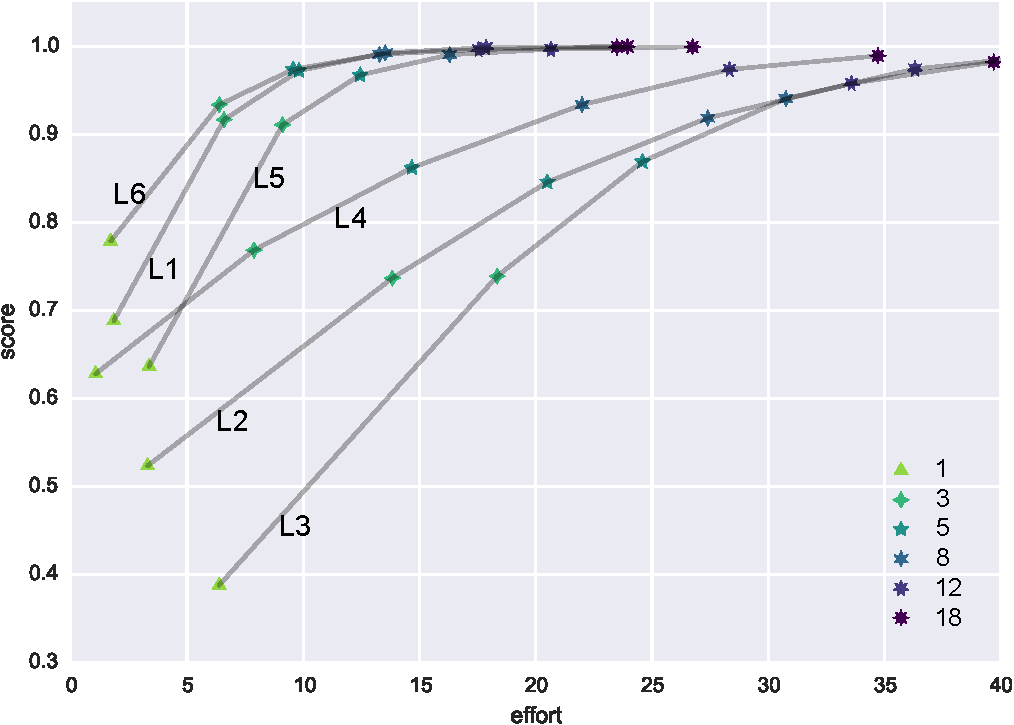
\includegraphics[width=.45\linewidth]{ncc-effort-score} & &
      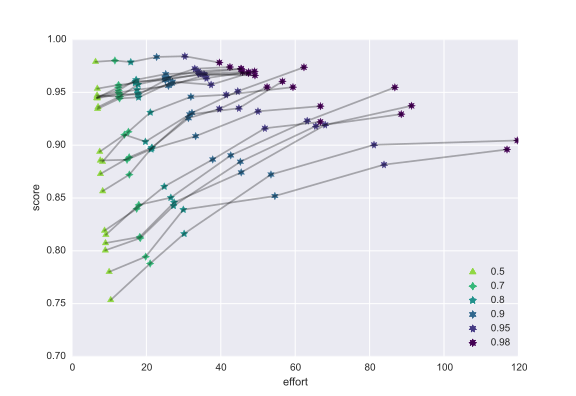
\includegraphics[width=.45\linewidth]{uc-effort-score}
    \end{tabular}
  \end{center}
\end{frame}

\begin{frame}
  \frametitle{Summary and Future Work}

  \begin{block}{}
    Use simple criteria, focus on input data and thresholds, not on models.
  \end{block}

  \medskip

  limitations and future work:
  \begin{itemize}
  \item multiple knowledge components
  \item wheel-spinning students
  \item forgetting
  \item partial credit
  \end{itemize}
\end{frame}


\end{document}